\documentclass{beamer}
\usetheme{metropolis}

% specifications for presenter mode
%\beamerdefaultoverlayspecification{<+->}
%\setbeamercovered{transparent}

\usepackage[english]{babel}
\usepackage[utf8x]{inputenc}

%\usepackage{coloremoji}
\usepackage{layout}
\usepackage{multirow}
\usepackage{array}
\usepackage{graphicx}
\graphicspath{ {Figs/} }

\setbeameroption{hide notes}
\setbeamertemplate{note page}[plain]
\usepackage{listings}
\usepackage{datetime}
\usepackage{url}
\usepackage{tcolorbox}
\usepackage{appendixnumberbeamer}

\usepackage{tikz}
\def\checkmark{\tikz\fill[scale=0.4](0,.35) -- (.25,0) -- (1,.7) -- (.25,.15) -- cycle;}

% math shorthand
\usepackage{bm}
\usepackage{amstext}
\usepackage{amsthm}
\usepackage{amsmath}
\usepackage{mathtools}
\newcommand{\R}{\mathbb{R}}
\newcommand{\D}{\mathcal{D}}
\newcommand{\E}{\mathbb{E}}
\newcommand{\I}{\mathbb{I}}
\newcommand{\pr}{\mathbb{P}}
\newcommand{\F}{\mathcal{F}}
\newcommand{\X}{\mathcal{X}}
\newcommand{\M}{\mathcal{M}}
\newcommand{\lik}{\mathcal{L}}

\newtheorem*{assumption*}{\assumptionnumber}
\providecommand{\assumptionnumber}{}
\makeatletter
\newenvironment{assumption}[2]
 {%
  \renewcommand{\assumptionnumber}{Assumption #1: $\mathcal{#2}$}%
  \begin{assumption*}%
  \protected@edef\@currentlabel{#1: $\mathcal{#2}$}%
 }
 {%
  \end{assumption*}
 }
\makeatother

\DeclarePairedDelimiterX{\infdivx}[2]{(}{)}{%
  #1\;\delimsize\|\;#2%
}
\newcommand{\infdiv}{D\infdivx}
\DeclarePairedDelimiter{\norm}{\lVert}{\rVert}
\DeclareMathOperator*{\argmin}{arg\,min}
\DeclareMathOperator*{\argmax}{arg\,max}

% indepndence notation macro
\newcommand\indep{\protect\mathpalette{\protect\independenT}{\perp}}
\def\independenT#1#2{\mathrel{\rlap{$#1#2$}\mkern2mu{#1#2}}}

% Bibliography
\usepackage{natbib}
\bibpunct{(}{)}{,}{a}{}{;}
\usepackage{bibentry}

% title info
\title{\normalsize Causal Inference and Variable Importance Analysis for
Continuous Quantities through Stochastic Interventions}

\subtitle{\scriptsize Considerations for two-phase sampling designs and open
source software\\[-10pt]}

\author{\href{https://nimahejazi.org}{Nima Hejazi}\\[-10pt]}

\institute{
  \begin{figure}[!htb]
    \centering
    \begin{minipage}{.65\textwidth}
        Group in Biostatistics, and \\
        Center for Computational Biology, \\
        University of California, Berkeley \\[6pt]
        
\includegraphics[scale=0.12]{twitter-icon.png}
          \href{https://twitter.com/nshejazi}{nshejazi} \\
        
\includegraphics[scale=0.09]{github-icon.png}
          \href{https://github.com/nhejazi}{nhejazi} \\
        
\includegraphics[scale=0.12]{homepage.png}
          \href{https://nimahejazi.org}{nimahejazi.org}
    \end{minipage}%
    \begin{minipage}{0.35\textwidth}
      \centering
      
\includegraphics[height=0.80in,width=0.80in]{ucberkeleyseal_874_540.eps}
    \end{minipage}
  \end{figure}
}

\date{\today}

%%%%%%%%%%%%%%%%%%%%%%%%%%%%%%%%%%%%%%%%%%%%%%%%%%%%%%%%%%%%%%%%%%%%%%%%%%%%%%%%

% Outline at beginning of each section
%\AtBeginSection[]
%{
  %\begin{frame}<beamer>
    %\frametitle{Outline}
    %\tableofcontents[currentsection]
  %\end{frame}
%}

%%%%%%%%%%%%%%%%%%%%%%%%%%%%%%%%%%%%%%%%%%%%%%%%%%%%%%%%%%%%%%%%%%%%%%%%%%%%%%%%

\begin{document}

\begin{frame}[noframenumbering]
  \thispagestyle{empty}
  \titlepage
\end{frame}

%%%%%%%%%%%%%%%%%%%%%%%%%%%%%%%%%%%%%%%%%%%%%%%%%%%%%%%%%%%%%%%%%%%%%%%%%%%%%%%%

\begin{frame}[c,noframenumbering]{Preview: Summary}
\thispagestyle{empty}

\begin{center}
\begin{itemize}
  \itemsep8pt
  \item Vaccine efficacy evaluation helps to develop enhanced vaccines better
    informed by biological properties of the target disease.
  \item HIV vaccines modulate immune responses as part of the mechanism for
    lowering HIV risk.
  \item \textit{Stochastic} interventions provide a flexible framework for
    considering \textbf{realistic} treatment policies.
  \item Large-scale vaccine trials often use two-phase sampling --- need to
    accommodate such designs.
  \item We've developed robust, open source statistical software for applying
    stochastic interventions in observational studies.
\end{itemize}
\end{center}

\note{This slide deck is for a short talk (about 30 minutes) on an approach to
  causal inference and nonparametric variable importance in the
  context of parameters defined as treatment shifts. Here, we introduce an
  additive treatment shift parameter, extensions for censored data (including
  a multiple double robustness property), new opensource statistical software
  for applying our approach, and applications to a vaccine efficacy trial
  examining HIV. This talk was most recently given as part of a student-run
  lunch seminar within the Division of Biostatistics at UC Berkeley.

}

\end{frame}

%%%%%%%%%%%%%%%%%%%%%%%%%%%%%%%%%%%%%%%%%%%%%%%%%%%%%%%%%%%%%%%%%%%%%%%%%%%%%%%%

\section{Motivations and Preliminaries}

%%%%%%%%%%%%%%%%%%%%%%%%%%%%%%%%%%%%%%%%%%%%%%%%%%%%%%%%%%%%%%%%%%%%%%%%%%%%%%%%

\begin{frame}[c]{Motivation: The Burden of HIV-1}

\begin{center}
\begin{itemize}
  \itemsep10pt
  \item HIV-1 epidemic is in its fourth decade, with 2.5 million new infections
    occurring annually worldwide.
  \item Though diminishing, number of newly infected persons outpaces number of
    patients starting antiretroviral therapy.
  \item As of 2013, progress is limited: the HIV vaccine efficacy trial with
    highest impact reported a 31\% reduction in infections.
  \item Careful study led to development of a targeted CD4+ and CD8+ T-cell and
    antibody boost vaccine, which underwent extensive pre-clinical and
    early-phase clinical testing.
\end{itemize}
\end{center}

\note{
}

\end{frame}

%%%%%%%%%%%%%%%%%%%%%%%%%%%%%%%%%%%%%%%%%%%%%%%%%%%%%%%%%%%%%%%%%%%%%%%%%%%%%%%%
\begin{frame}[c]{Motivation: The HVTN 505 Trial}

\begin{center}
\begin{itemize}
  \itemsep10pt
  \item The HIV Vaccine Trials Network (HVTN) 505 preventive vaccine efficacy
    trial, detailed in \cite{hammer2013efficacy}.
  \item $n = 2504$ participants --- all observed cases matched to controls after
    collection of endpoints of interest.
  \item Baseline variables ($W$): sex, age, BMI, SES, etc.
  \item Variables of interest ($A$): immune response markers (post-vaccination
    T-cell activity).
  \item Outcome of interest ($Y$): HIV-1 infection status.
  \item The 505 trial includes both vaccine and placebo arms --- we focus on
    only the vaccine arm (for now).
\end{itemize}
\end{center}

\note{
\begin{itemize}
  \itemsep10pt
  \item A vaccine effective at preventing HIV-1 acquisition would be a
    cost-effective and durable approach to halting the worldwide epidemic.
  \item Identifying vaccine-induced immune-response biomarkers that predict a
    vaccine's ability to protect individuals from HIV-1 infection is a high
    priority.
  \item The study was halted on 22 April 2013 due to absence of vaccine
    efficacy. There was no significant effect of the vaccine on the primary
    infection endpoint of HIV-1 infection between week 28 and month 24.
\end{itemize}
}

\end{frame}

%%%%%%%%%%%%%%%%%%%%%%%%%%%%%%%%%%%%%%%%%%%%%%%%%%%%%%%%%%%%%%%%%%%%%%%%%%%%%%%%

\begin{frame}[c]{Motivation: Enhanced Vaccines for HIV-1}

\begin{center}
\begin{itemize}
  \itemsep10pt
  \item \textbf{Question}: How would changes in immune response profile (for a
    given marker) impact HIV-1 infection?
  \item Using observational data, thought experiments will allow us to examine
    scenarios where immune responses were tweaked differently by a given
    vaccine.
  \item By isolating potential immune response targets, improved vaccines can be
    constructed with such targets in mind.
  \item \textbf{Conclusion:} Understanding which immune responses impact vaccine
    efficacy helps develop more efficacious vaccines.
\end{itemize}
\end{center}

\note{
\begin{itemize}
  \itemsep10pt
  \item HIV is a high-impact public health issue but numerous attempts to
    develop vaccines have met with only mild success.
  \item The complexity of the disease mechanism makes it quite challenging to
    study the numerous factors that contribute to a possible mitigation of
    infection risk.
\end{itemize}
}

\end{frame}

%%%%%%%%%%%%%%%%%%%%%%%%%%%%%%%%%%%%%%%%%%%%%%%%%%%%%%%%%%%%%%%%%%%%%%%%%%%%%%%%

\begin{frame}[c]{Structure of the Full Data}

\begin{center}
\begin{itemize}
  \itemsep10pt
  \item Consider $X = (W, A, Y) \sim P_0^X \in \mathcal{M}^X_{NP}$
    \begin{itemize}
      \itemsep6pt
      \item $W$ --- baseline covariates (e.g., sex, age, etc.),
      \item $A$ --- intervention (e.g., immune response profile
        post-vaccination),
      \item $Y$ --- outcome of interest (e.g., HIV-1 infection status),
      \item $P_0^X$ --- true (unknown) distribution of the full data $X$,
      \item $\mathcal{M}^X_{NP}$ --- nonparametric statistical model.
    \end{itemize}
  \item Consider observing $X_1, \ldots, X_n$, i.e., $n$ iid copies of $X$.
  \item For now, ignore two-phase sampling design of HVTN 505.
\end{itemize}
\end{center}

\note{
}

\end{frame}

%%%%%%%%%%%%%%%%%%%%%%%%%%%%%%%%%%%%%%%%%%%%%%%%%%%%%%%%%%%%%%%%%%%%%%%%%%%%%%%%

\begin{frame}[c]{Likelihood Factorization for the Full Data}

\begin{center}
\begin{itemize}
  \itemsep10pt
  \item Let $q_{0, Y}$ be the conditional density of $Y$ given $(A, W)$ wrt
    dominating measure $\xi$.
  \item Let $q_{0, A}$ be the conditional density of $A$ given $W$ wrt
    dominating measure $\mu$.
  \item Let $q_{0, W}$ be the density of $W$ wrt dominating measure $\nu$.
  \item Then, for $p_0^X$, density of $X$ wrt the product measure, density
    evaluated on a particular observation $x$:
    \begin{equation*}\label{likelihood_factorization}
       p_0^X(x) = q^X_{0,Y}(y \mid A = a, W = w) q^X_{0,A}(a \mid W = w)
        q^X_{0,W}(w).
     \end{equation*}
\end{itemize}
\end{center}

\note{
}

\end{frame}

%%%%%%%%%%%%%%%%%%%%%%%%%%%%%%%%%%%%%%%%%%%%%%%%%%%%%%%%%%%%%%%%%%%%%%%%%%%%%%%%

\begin{frame}[c]{NPSEM for the Full Data}

\begin{center}
\begin{itemize}
  \itemsep10pt
  \item Use a nonparametric structural equation model (NPSEM) to describe
    generation of $X$ \citep{pearl2009causality}, specifically
    \begin{align*}
      W &= f_W(U_W) \\ A &= f_A(W, U_A) \\ Y &= f_Y(A, W, U_Y)
    \end{align*}
  \item NPSEM parameterizes $p_0^X$ in terms of the distribution of RVs $(X, U)$
    modeled by this system of equations.
  \item Implies a model for the distribution of counterfactual RVs generated by
    interventions on the data-generating process.
\end{itemize}
\end{center}

\note{
\begin{itemize}
  \item Notation: let $f_W$, $f_A$, $f_Y$ be deterministic functions, and $U_W$,
    $U_A$, $U_Y$ exogenous RVs.
\end{itemize}
}

\end{frame}

%%%%%%%%%%%%%%%%%%%%%%%%%%%%%%%%%%%%%%%%%%%%%%%%%%%%%%%%%%%%%%%%%%%%%%%%%%%%%%%%

\begin{frame}[c]{Interlude: On Realism and Causal Inference}

\begin{center}
\begin{itemize}
  \itemsep6pt
  \item Our motivations, again: How do changes in a given immune response affect
    post-vaccination risk of HIV-1 infection?
  \item How does \textit{intervening} on a given immune response \textit{cause}
    changes in HIV-1 risk? How can future vaccines be informed by the lessons
    we can learn from such thought experiments?
  \item What does it mean to intervene on a continous-valued quantity? Should
    one consider setting a specific value deterministically? Perhaps with a
    dynamic intervention?
  \item Immune responses are surely functions of $W$, and, perhaps, a posited
    change should depend on $A$ as well.
\end{itemize}
\end{center}

\note{
  Classical parameters from causal inference (e.g., ATE) are not well-suited for
  such questions.
}

\end{frame}

%%%%%%%%%%%%%%%%%%%%%%%%%%%%%%%%%%%%%%%%%%%%%%%%%%%%%%%%%%%%%%%%%%%%%%%%%%%%%%%%

\section{Science $\times$ Software $\times$ Statistics}

%%%%%%%%%%%%%%%%%%%%%%%%%%%%%%%%%%%%%%%%%%%%%%%%%%%%%%%%%%%%%%%%%%%%%%%%%%%%%%%%

\begin{frame}[c]{Statistical Software Promotes Scientific Reproducibility}

\begin{center}

\begin{tcolorbox}
  ``The origins of the scientific method$\ldots$ amount to insistence on
  direct evdience. This is reflected in the motto of The Royal Society, founded
  in 1660: \textit{Nullius in verba}, which roughly means `take nobody's word
  for it'.'' ---Philip B.~Stark, in \textit{The Practice of Reproducible
  Research}
\end{tcolorbox}

\begin{itemize}
  \itemsep4pt
  \item \textit{Show me}, not \textit{trust me} --- robust, well documented,
    rigorously tested software allows others to directly assess our claims.
  \item The software we distribute allows others to engage with our analysis of
    the HVTN 505 trial and to apply our method to similar vaccine efficacy
    trials.
  \item We will be making \textit{causal} claims about vaccine efficacy. Our
    results could be medically impactful, so reproducibility is vital.
\end{itemize}
\end{center}

\note{
}

\end{frame}

%%%%%%%%%%%%%%%%%%%%%%%%%%%%%%%%%%%%%%%%%%%%%%%%%%%%%%%%%%%%%%%%%%%%%%%%%%%%%%%%

\begin{frame}[c]{What's wrong with that code I wrote that one time?}

\begin{center}

\begin{tcolorbox}
  ``An article$\ldots$in a scientific publication is not the scholarship itself,
  it is merely advertising of the scholarship. The actual scholarship is the
  complete software development environment and the complete set of instructions
  which generated the figures.'' ---David Donoho, on \textit{WaveLab}
\end{tcolorbox}

\begin{itemize}
  \item Reproducible applied statistics \textit{requires robust software}:
    \begin{itemize}
      \itemsep4pt
      \item Clear, easily acessible documentation, including examples.
      \item Unit testing to rigorously assess functions, classes, etc.
      \item Continuous integration, ensuring accessibility across systems and
        constant monitoring of software quality.
      \item Open source development, embodying an ongoing, continuous, public
        peer review of the software product.
    \end{itemize}
\end{itemize}
\end{center}

\note{
\begin{itemize}
  \itemsep4pt
  \item Statistical publications feature simulation and data analytic results,
    largely insufficient for rigorously assessing claims.
  \item ``\textit{A Year is a Long Time in this Business.} Once, about a year
    after one of us had done some work and written an article (and basically
    forgot the details of the work he had done), he had the occasion to apply
    the methods of the article on a newly-arrived dataset. When he went back to
    the old software library to try and do it, he couldn't remember how the
    software worked --- invocation sequences, data structures, etc. In the end,
    he abandoned the project, saying he just didn't have time to get in to it
    anymore.'' ---from \textit{WaveLab}
  \item Another example (also from \textit{WaveLab}): this one about how the
    figures in an interesting paper were produced by software built by the
    authors, but the authors themselves did not remember the parameter settings
    that produced the nice figure, so they just hoped that the configuration
    would come back to them some time later.
\end{itemize}
}

\end{frame}

%%%%%%%%%%%%%%%%%%%%%%%%%%%%%%%%%%%%%%%%%%%%%%%%%%%%%%%%%%%%%%%%%%%%%%%%%%%%%%%%

\begin{frame}[c]{Software Ecosystem --- The \texttt{tlverse}!}

\begin{figure}[H]
  \centering
  
\includegraphics[width=\textwidth]{tlverse}
  \caption{
    \url{https://github.com/tlverse}
  }
\end{figure}

\vspace{-1em}

\begin{center}
\begin{itemize}
  \itemsep4pt
  \item A new software environment and framework for Targeted Learning, with a
    focus on extensibility.
  \item \textit{Goal:} expose a set of design principles off of which all future
    Targeted Learning software will be built.
  \item \textit{How?} A core framework, plus minimal extensions (``connector
    packages''), each implementing a few estimators.
\end{itemize}
\end{center}

\note{
\begin{itemize}
  \itemsep10pt
  \item Contribute on GitHub: \url{https://github.com/tlverse}.
  \item Reach out to us with questions and any feature requests.
\end{itemize}
}

\end{frame}

%%%%%%%%%%%%%%%%%%%%%%%%%%%%%%%%%%%%%%%%%%%%%%%%%%%%%%%%%%%%%%%%%%%%%%%%%%%%%%%%

\section{Towards Stochastic Interventions}

%%%%%%%%%%%%%%%%%%%%%%%%%%%%%%%%%%%%%%%%%%%%%%%%%%%%%%%%%%%%%%%%%%%%%%%%%%%%%%%%

\begin{frame}[c]{Static or Dynamic Interventions in our NPSEM}

\begin{center}
\begin{itemize}
  \itemsep10pt
  \item A \textit{static intervention} replaces $f_A$ with a specific value $a$
    in the support of $q_{0, A}(\cdot \mid W)$ a.e.~$q_{0,W}$.
  \item This requires specifying a particular value of the intervention (i.e.,
    $A = a$) under which to evaluate the outcome.
  \item Is it really sensible to set the value of an immune response to a
    particular value? (Even as a function of $W$.)
  \item This is statistically accessible but scientifically uninteresting
    (perhaps dishonest, even) --- one would have to test many different values
    $a$, with only intuition as a guide.
\end{itemize}
\end{center}

\note{
  \begin{itemize}
    \item We'd like to posit changes to immune responses that we can actually
      induce.
    \item We can mathematically consider the counterfactual of setting an immune
      response to a specific value, but we cannot do this in practice --- thus,
      it is rather uninteresting.
    \item Instead, we consider counterfactuals that might come to pass. We are
      able to create vaccines that alter the level of an immune response by a
      small amount.
  \end{itemize}
}

\end{frame}

%%%%%%%%%%%%%%%%%%%%%%%%%%%%%%%%%%%%%%%%%%%%%%%%%%%%%%%%%%%%%%%%%%%%%%%%%%%%%%%%

\begin{frame}[c]{Interlude: A Linear Modeling Perspective}

\begin{center}
\begin{itemize}
  \itemsep6pt
  \item Briefly consider a simple data structure: $X = (Y, A)$; we seek to model
    the outcome $Y$ as a function of $A$.
  \item To posit a linear model, consider $Y_i = \beta_0 + \beta_1 A_i +
    \epsilon_i$, with error $\epsilon_i \sim N(0, 1)$.
  \item Letting $\delta$ be a change in $A$, $Y_{A + \delta} - Y_A$ may be
    expressed
    \begin{align*}
      \E Y_{A + \delta} - \E Y_A &= [\beta_0 + \beta_1 (\E A + \delta)] -
        [\beta_0 + \beta_1 (\E A)] \\
        &= \beta_0 - \beta_0 + \beta_1 \E A - \beta_1 \E A + \beta_1 \delta \\
        &= \beta_1 \delta
    \end{align*}
  \item Thus, a \textit{unit shift} in $A$ (i.e., $\delta = 1$) may be seen as
    inducing a change in the difference in outcomes of magnitude $\beta_1$.
\end{itemize}
\end{center}

\note{
  \begin{itemize}
    \item We extend this result to the mean counterfactual outcomes under the
      nonparametric model $\M$.
    \item Linear modeling analogy re: conversation with Alan on 22 August.
  \end{itemize}
}

\end{frame}

%%%%%%%%%%%%%%%%%%%%%%%%%%%%%%%%%%%%%%%%%%%%%%%%%%%%%%%%%%%%%%%%%%%%%%%%%%%%%%%%

\begin{frame}[c]{Stochastic Interventions in our NPSEM}

\begin{center}
\begin{itemize}
  \itemsep8pt
  \item \textit{Stochastic interventions} modify the value $A$ would naturally
    assume, $f_A(W, U_A)$, by drawing from a modified intervention distribution
    $G^*(\cdot \mid W)$ so that the new value $A^* \sim G^*(\cdot \mid W)$.
  \item This generates a counterfactual RV, with distribution $P_{0}^d$,
    $Y_{d(A, W)} \coloneqq f_Y(d(A,W), W, U_Y) \equiv Y_{G^*} \coloneqq
    f_Y(A^*, W, U_Y)$.
  \item We estimate $\psi_{0, d} \coloneqq \E_{P_0^d}\{Y_{d(A,W)}\}$, mean of
    $Y_{d(A, W)}$.
  \item For HVTN 505, $\psi_{0,d}$ is the counterfactual risk of HIV-1
    infection, had the observed value of the immune response been altered under
    the rule $d(A,W)$ defining $G^*(\cdot \mid W)$.
  \item Helps isolate immune responses that causally inhibit HIV-1; future
    vaccines may be designed to target these markers.
\end{itemize}
\end{center}

\note{
  \begin{itemize}
    \item Several different ways to consider stochastic interventions.
    \item Starts with Mark and Ivan's simple stochastic shift.
    \item Extensions to modified treatment policies.
    \item The new value of $A$ may be denoted $A^* \sim G^*(\cdot \mid W)$,
      where $A^* = d(W, U^*)$ for a rule $d$ and random error $U^*$.
  \end{itemize}
}

\end{frame}

%%%%%%%%%%%%%%%%%%%%%%%%%%%%%%%%%%%%%%%%%%%%%%%%%%%%%%%%%%%%%%%%%%%%%%%%%%%%%%%%

\begin{frame}[c]{From the Causal to the Statistical Target Parameter}

\begin{center}
\begin{tcolorbox}
\begin{assumption}{1}{\textit{Consistency}}\label{consistency}
  $Y^{d(a_i, w_i)}_i = Y_i$ in the event $A_i = d(a_i, w_i)$, for
  $i = 1, \ldots, n$
\end{assumption}
\end{tcolorbox}

\begin{tcolorbox}
\begin{assumption}{2}{\textit{SUTVA}}\label{sutva}
  $Y^{d(a_i, w_i)}_i$ does not depend on $d(a_j, w_j)$ for $i = 1,
  \ldots, n$ and $j \neq i$, or lack of interference
  \citep{rubin1978bayesian, rubin1980randomization}
\end{assumption}
\end{tcolorbox}

\begin{tcolorbox}
\begin{assumption}{3}{\textit{Strong ignorability}}\label{ignorability}
  $A_i \indep Y^{d(a_i, w_i)}_i \mid W_i$, for $i = 1, \ldots, n$
\end{assumption}
\end{tcolorbox}
\end{center}

\note{
}

\end{frame}

%%%%%%%%%%%%%%%%%%%%%%%%%%%%%%%%%%%%%%%%%%%%%%%%%%%%%%%%%%%%%%%%%%%%%%%%%%%%%%%%

\begin{frame}[c]{From the Causal to the Statistical Target Parameter}

\begin{center}
\begin{tcolorbox}
\begin{assumption}{4}{\textit{Positivity (or overlap)}}\label{positivity}
  $a_i \in \mathcal{A} \implies d(a_i, w_i) \in \mathcal{A}$ for all
  $w \in \mathcal{W}$, where $\mathcal{A}$ denotes the support of $A$
  conditional on $W = w_i$ for all $i = 1, \ldots n$
\end{assumption}
\end{tcolorbox}

\begin{itemize}
  \itemsep4pt
  \item This positivity assumption is not quite the same as that required for
    categorical interventions.
  \item In particular, we do not require that the intervention density place
    mass across all strata defined by $W$.
  \item Rather, we merely require the post-intervention quantity be seen in the
    observed data for given $a_i \in \mathcal{A}$ and $w_i \in \mathcal{W}$.
\end{itemize}
\end{center}

\note{
}

\end{frame}

%%%%%%%%%%%%%%%%%%%%%%%%%%%%%%%%%%%%%%%%%%%%%%%%%%%%%%%%%%%%%%%%%%%%%%%%%%%%%%%%

\begin{frame}[c]{Statistical Target Parameter for Shift Interventions}

\begin{center}
\begin{itemize}
  \itemsep10pt
  \item We have the statistical functional (target parameter)
    \citep{diaz2012population}:
    \begin{equation*}
      \Psi(P_0^X) = \E_{P_0^X}{\overline{Q}(d(A, W), W)},
    \end{equation*}
    allowing estimation of causal parameter $\psi_{0,d} = \E Y_{d(A, W)}$.
  \item We now seek to efficiently estimate this target parameter in the
    nonparametric model $\M$.
  \item We implement a targeted minimum loss-based estimator of this statistical
    target parameter.
\end{itemize}
\end{center}

\note{
  \begin{itemize}
    \item Note that $\overline{Q}(\cdot \mid W)$ is properly referred to as a
      \textit{functional of the likelihood}.
  \end{itemize}
}

\end{frame}

%%%%%%%%%%%%%%%%%%%%%%%%%%%%%%%%%%%%%%%%%%%%%%%%%%%%%%%%%%%%%%%%%%%%%%%%%%%%%%%%

\begin{frame}[c]{Targeted Minimum Loss-Based Estimation}

\begin{center}
\begin{itemize}
  \itemsep10pt
  \item A TMLE is an algorithm for updating initial estimators so as to satisfy
    an arbitrary set of estimating equations.
  \item Semiparametric-efficient estimation thru solving efficient influence
    function estimating equation wrt the model $\M$.
  \item Statistical target parameter:
    $\Psi(P_0^X) = \E_{P_0^X}{\overline{Q}(d(A, W), W)}$
  \item For which the efficient influence function (EIF) is
    \begin{equation*}
      D(P_0^X)(x) = H(a, w)({y - \overline{Q}(a, w)}) +
      \overline{Q}(d(a, w), w) - \Psi(P_0^X)
    \end{equation*}
  \item The auxiliary covariate $H(a,w)$ may be expressed
    \begin{equation*}
      H(a,w) = \I(a + \delta < u(w)) \frac{g_0(a - \delta \mid w)}
      {g_0(a \mid w)} + \I(a + \delta \geq u(w))
    \end{equation*}
\end{itemize}
\end{center}

\note{
  \begin{itemize}
    \item The auxiliary covariate simplifies when the treatment is in the limits
      (conditional on $W$) --- i.e., for $A_i \in (u(w) - \delta, u(w))$, then
      we have $H(a,w) = \frac{g_0(a - \delta \mid w)}{g_0(a \mid w)} + 1$.
    \item Need to explicitly remind the audience what $u(w)$ is again. It's only
      appeared once at this point, and only been mentioned in passing.
  \end{itemize}
}

\end{frame}

%%%%%%%%%%%%%%%%%%%%%%%%%%%%%%%%%%%%%%%%%%%%%%%%%%%%%%%%%%%%%%%%%%%%%%%%%%%%%%%%

\begin{frame}[c]{Key Properties of TML Estimators}

\begin{center}
\begin{itemize}
  \itemsep10pt
  \item \textbf{Asymptotic linearity:}
    \begin{equation*}
      \Psi(P_n^*) - \Psi(P_0^X) = \frac{1}{n} \sum_{i = 1}^{n} D(P_0^X)(X_i) +
      o_P\left(\frac{1}{\sqrt{n}}\right)
    \end{equation*}
  \item \textbf{Gaussian limiting distribution:}
    \begin{equation*}
      \sqrt{n}(\Psi(P_n^*) - \Psi(P_0^X)) \to N(0, Var(D(P_0^X)(X)))
    \end{equation*}
  \item \textbf{Statistical inference:}
    \begin{equation*}
      \text{Wald-type CI}: \Psi(P_n^*) \pm z_{\alpha} \cdot
      \frac{\sigma_n}{\sqrt{n}},
    \end{equation*}
    where $\sigma_n^2$ is computed directly via
    $\sigma_n^2 = \frac{1}{n} \sum_{i = 1}^{n} D^2(\cdot)(X_i)$.
\end{itemize}
\end{center}

\note{
Under the additional condition that the remainder term $R(\hat{P}^*, P_0)$
decays as $o_P \left( \frac{1}{\sqrt{n}} \right),$ we have that
$\Psi_n - \Psi_0 = (P_n - P_0) \cdot D(P_0) + o_P
\left( \frac{1}{\sqrt{n}} \right),$ which, by a central limit theorem,
establishes a Gaussian limiting distribution for the estimator, with variance
$V(D(P_0))$, the variance of the efficient influence function
when $\Psi$ admits an asymptotically linear representation.

The above implies that $\Psi_n$ is a $\sqrt{n}$-consistent estimator of $\Psi$,
that it is asymptotically normal (as given above), and that it is locally
efficient. This allows us to build Wald-type confidence intervals, where
$\sigma_n^2$ is an estimator of $V(D(P_0))$. The estimator $\sigma_n^2$
may be obtained using the bootstrap or computed directly via
$\sigma_n^2 = \frac{1}{n} \sum_{i = 1}^{n} D^2(\bar{Q}_n^*, g_n)(O_i)$

We obtain semiparametric-efficient estimation and robust inference in the
nonparametric model $\M$ by solving the efficient influence function.

\begin{enumerate}
   \item If $D(\bar{Q}_n^*, g_n)$ converges to $D(P_0)$ in $L_2(P_0)$ norm.
   \item The size of the class of functions $\bar{Q}_n^*$ and $g_n$ is bounded
     (technically, $\exists \mathcal{F}$ st
     $D(\bar{Q}_n^*, g_n) \in \mathcal{F}$ whp, where $\mathcal{F}$ is a
     Donsker class)
\end{enumerate}
}

\end{frame}

%%%%%%%%%%%%%%%%%%%%%%%%%%%%%%%%%%%%%%%%%%%%%%%%%%%%%%%%%%%%%%%%%%%%%%%%%%%%%%%%

\begin{frame}[c]{Algorithm for TML Estimation}

\begin{center}
\begin{enumerate}\label{tmle_algo}
  \itemsep6pt
  \item Construct initial estimators $g_n$ of $g_0(A, W)$ and $Q_n$ of
    $\overline{Q}_0(A, W)$, perhaps using data-adaptive regression techniques.
  \item For each observation $i$, compute an estimate $H_n(a_i, w_i)$ of the
    auxiliary covariate $H(a_i,w_i)$.
  \item Estimate the parameter $\epsilon$ in the logistic regression model
    $$ \text{logit}\overline{Q}_{\epsilon, n}(a, w) =
    \text{logit}\overline{Q}_n(a, w) + \epsilon H_n(a, w),$$
    or an alternative regression model incorporating weights.
  \item Compute TML estimator $\Psi_n$ of the target parameter, defining update
    $\overline{Q}_n^{\star}$ of the initial estimate
    $\overline{Q}_{n, \epsilon_n}$:
    \begin{equation*}\label{tmle}
      \Psi_n = \Psi(P_n^*) = \frac{1}{n} \sum_{i = 1}^n
        \overline{Q}_n^{\star}(d(A_i, W_i), W_i).
      \end{equation*}
\end{enumerate}
\end{center}

\note{
  \begin{itemize}
    \item We recommend using nonparametric methods for the initial estimators,
      as consistent estimation is necessary for efficiency of the estimator
      $\Psi_n$.
    \item Intuition for the submodel fluctuation?
  \end{itemize}
}

\end{frame}

%%%%%%%%%%%%%%%%%%%%%%%%%%%%%%%%%%%%%%%%%%%%%%%%%%%%%%%%%%%%%%%%%%%%%%%%%%%%%%%%

\begin{frame}[c]{Software package: \texttt{R}/\texttt{sl3}}

\begin{figure}[H]
  \centering
  
\includegraphics[width=\textwidth]{sl3}
  \caption{
    \url{https://github.com/tlverse/sl3}
  }
\end{figure}

\vspace{-2em}

\begin{center}
\begin{itemize}
  \itemsep4pt
  \item A robust and efficient implementation of the Super Learner algorithm,
    drawing on the concept of pipelines popularized by \texttt{scikit-learn}
    (\url{http://scikit-learn.org/stable/}).
  \item The first software package and one of the core engines of the
    \texttt{tlverse} ecosystem.
\end{itemize}
\end{center}

\note{
\begin{itemize}
  \itemsep10pt
  \item Contribute on GitHub: \url{https://github.com/tlverse/sl3}.
  \item Reach out to us with questions and any feature requests.
\end{itemize}
}

\end{frame}

%%%%%%%%%%%%%%%%%%%%%%%%%%%%%%%%%%%%%%%%%%%%%%%%%%%%%%%%%%%%%%%%%%%%%%%%%%%%%%%%

\begin{frame}[c]{Simulation Study: TML Estimation}

\begin{center}
\begin{itemize}
  \itemsep6pt
  \item For a single observational unit $X = (W, A, Y)$, data are simulated
    using the following set of structural equations:
    \begin{align*}
      W & \sim Bern(p = 0.5)\\
      A & \sim N(\mu = \gamma \cdot W, \sigma^2 = 1)\\
      Y & = A + W + \epsilon,
     \end{align*}
   \item Let $\gamma = 2$ be a multiplier of the effect of the baseline
     covariate $W$ on the natural value of the treatment $A$, and white noise
     $\epsilon \sim N(0, 1)$.
   \item We consider the case of observing a data structure composed of $n$
     replicates of $X$, i.e., $X_1, \ldots, X_n$.
   \item Letting $\delta = 0.5$, we construct a TML estimate of the
     counterfactual mean outcome $\psi_{0, d}$.
\end{itemize}
\end{center}

\note{
\begin{itemize}
 \item Sample sizes $n_{\text{samp}} \in \{50, 250, 1000, 2000\}$, each with
   $n_{\text{sim}} = 1000$ simulations were performd at each sample size.
\end{itemize}
}

\end{frame}

%%%%%%%%%%%%%%%%%%%%%%%%%%%%%%%%%%%%%%%%%%%%%%%%%%%%%%%%%%%%%%%%%%%%%%%%%%%%%%%%

\begin{frame}[c]{Simulation Study: TML Estimation}

\vspace{-0.45em}
\begin{figure}\label{fig:tmle3shift-bias}
  \centering
  \includegraphics[scale=0.47]{tmle3shift-sims/bias_plot}
\end{figure}

\note{
}

\end{frame}

%%%%%%%%%%%%%%%%%%%%%%%%%%%%%%%%%%%%%%%%%%%%%%%%%%%%%%%%%%%%%%%%%%%%%%%%%%%%%%%%

\begin{frame}[c]{Simulation Study: TML Estimation}

\vspace{-0.45em}
\begin{figure}\label{fig:tmle3shift-mcvar}
  \centering
  \includegraphics[scale=0.47]{tmle3shift-sims/mc_var_plot}
\end{figure}

\note{
}

\end{frame}

%%%%%%%%%%%%%%%%%%%%%%%%%%%%%%%%%%%%%%%%%%%%%%%%%%%%%%%%%%%%%%%%%%%%%%%%%%%%%%%%

\begin{frame}[c]{Simulation Study: TML Estimation}

\vspace{-0.45em}
\begin{figure}\label{fig:tmle3shift-avgse}
  \centering
  \includegraphics[scale=0.47]{tmle3shift-sims/se_avg_plot}
\end{figure}

\note{
}

\end{frame}

%%%%%%%%%%%%%%%%%%%%%%%%%%%%%%%%%%%%%%%%%%%%%%%%%%%%%%%%%%%%%%%%%%%%%%%%%%%%%%%%

\begin{frame}[c]{Software package: \texttt{R}/\texttt{tmle3shift}}

\begin{figure}[H]
  \centering
  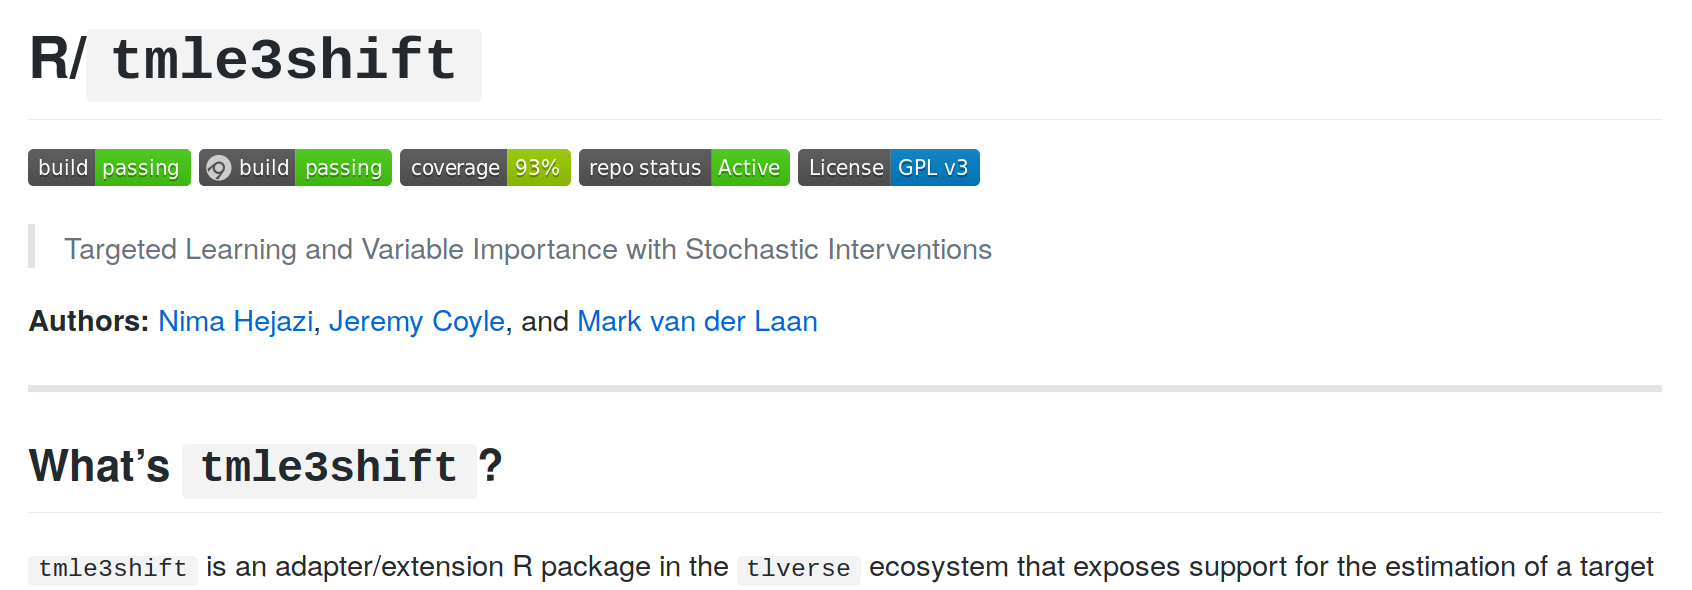
\includegraphics[width=\textwidth]{tmle3shift}
  \caption{
    \url{https://github.com/tlverse/tmle3shift}
  }
\end{figure}

\vspace{-2em}

\begin{center}
\begin{itemize}
  \itemsep4pt
  \item Tools for assessing the effects of stochastic interventions.
  \item Supports interventions that enforce positivity constraints.
  \item First of many ``connector'' \texttt{R} packages that extend the
    \texttt{tlverse} ecosystem.
\end{itemize}
\end{center}

\note{
\begin{itemize}
  \itemsep10pt
  \item Contribute on GitHub: \url{https://github.com/tlverse/tmle3shift}.
  \item Reach out to us with questions and any feature requests.
\end{itemize}
}

\end{frame}

%%%%%%%%%%%%%%%%%%%%%%%%%%%%%%%%%%%%%%%%%%%%%%%%%%%%%%%%%%%%%%%%%%%%%%%%%%%%%%%%

\section{Two-Phase Sampling Designs}

%%%%%%%%%%%%%%%%%%%%%%%%%%%%%%%%%%%%%%%%%%%%%%%%%%%%%%%%%%%%%%%%%%%%%%%%%%%%%%%%

\begin{frame}[c]{Data Structure for Two-Phase Designs}

\begin{center}
\begin{itemize}
  \itemsep8pt
  \item In the 505 HIV-1 trial, all infected individuals are matched to controls
    after endpoints are collected.
  \item We need to extend our full data structure $X = (W,A,Y)$ to accommodate
    such a sampling procedure.
  \item Consider the observed data structure $O = (W, \Delta, \Delta A, Y)$, a
    masked version of the full data structure.
  \item Let $\Delta = f(Y, W)$ be binary s.t.~$\Delta \in \{0, 1\}$, where
    $\Delta = 1$ corresponds to being selected into the second-stage sample.
  \item Let $\pi_0(Y,W) = \pr(\Delta = 1 \mid Y,W)$, and let $\pi_n(Y,W)$ be an
    estimator of $\pi_0(Y,W)$.
\end{itemize}
\end{center}

\note{
  \begin{itemize}
    \item Note that matching is done based on $\{W, Y\}$.
  \end{itemize}
}

\end{frame}

%%%%%%%%%%%%%%%%%%%%%%%%%%%%%%%%%%%%%%%%%%%%%%%%%%%%%%%%%%%%%%%%%%%%%%%%%%%%%%%%

\begin{frame}[c]{Augmented Estimators for Two-Phase Designs}

\begin{center}
\begin{itemize}
  \itemsep10pt
  \item \cite{rose2011targeted2sd} introduce the IPCW-TMLE, to be used when
    observed data is subject to two-phase sampling.
  \item Their proposal constructs estimators for an observed data structure of
    the form $O = (V, \Delta, \Delta X)$.
  \item In our use-case, the sampling node $V = \{Y, W\}$, and thus we have our
    proposed data structure $O = (W, \Delta, \Delta A, Y)$.
  \item \textit{Initial proposal:} correct for two-phase sampling by using an
    IPC-weighted loss function:
    \begin{equation*}
      \lik(P_0^X)(O) = \frac{\Delta}{\pi_n(Y, W)}\lik^F(P_0^X)(X)
    \end{equation*}
\end{itemize}
\end{center}

\note{
}

\end{frame}

%%%%%%%%%%%%%%%%%%%%%%%%%%%%%%%%%%%%%%%%%%%%%%%%%%%%%%%%%%%%%%%%%%%%%%%%%%%%%%%%

\begin{frame}[c]{Efficiency Under Two-Phase Sampling}

\begin{center}
\begin{itemize}
  \itemsep10pt
  \item When the sampling mechanism is not known by design, it is best to employ
    a nonparametric estimator of $\pi_0(Y, W)$.
  \item When $\pi_0(Y, W)$ is estimated nonparametrically, the IPCW augmentation
    must be applied to the EIF:
    \begin{align*}
      D(P_0^X)(o) &= \frac{\Delta}{\pi_0(y, w)} D^F(P_0^X)(x) \\&- \left(1 -
        \frac{\Delta} {\pi_0(y, w)}\right)\E(D^F(P_0^X)(x) \mid
        \Delta = 1, Y = y, W = w),
    \end{align*}
    expressed in terms of the full data EIF $D^F(P_0^X)(x)$.
\end{itemize}
\end{center}

\note{
}

\end{frame}

%%%%%%%%%%%%%%%%%%%%%%%%%%%%%%%%%%%%%%%%%%%%%%%%%%%%%%%%%%%%%%%%%%%%%%%%%%%%%%%%

\begin{frame}[c]{Efficiency Under Two-Phase Sampling}

\begin{center}
  \textbf{The IPC-augmented EIF points out two distinct terms:}
  \begin{tcolorbox}
    $\frac{\Delta}{\pi_0(y, w)}D^F(P_0^X)(x)$
  \end{tcolorbox}
  The IPC-weighted EIF of the full data structure $X$, relative to the
  nonparametric model $\M$; and,
  \vspace{1em}
  \begin{tcolorbox}
    $\left(1 - \frac{\Delta}{\pi_0(y, w)}\right)$ $\E(D^F(P_0^X)(x) \mid
      \Delta = 1, Y = y, W = w)$
  \end{tcolorbox}
  The expectation of the full data EIF $D^F(P_0^X)(x)$, taken only over units
  selected by the sampling mechanism (i.e., $\Delta = 1$).
\end{center}

\note{
}

\end{frame}

%%%%%%%%%%%%%%%%%%%%%%%%%%%%%%%%%%%%%%%%%%%%%%%%%%%%%%%%%%%%%%%%%%%%%%%%%%%%%%%%

\begin{frame}[c]{Emergent Property: Multiple Robustness}

\begin{center}
\begin{itemize}
  \itemsep10pt
  \item We now have a semiparametric-efficient and robust procedure for
    assessing the effect of the intervention $d(a,w) = a + \delta$.
  \item Due to the construction of the IPCW-TMLE, the resultant estimator is
    robust and efficient under two-phase sampling.
  \item Uniquely, a multiple robustness property emerges --- through
    combinations of $(g, Q)$ and $(\pi(Y, W), \E(D^F(P^X_0)(x) \mid Y, W))$.
  \item This allows us to assess how posited shifts in the assayed immune
    responses would have affected HIV-1 infection risk.
\end{itemize}
\end{center}

\note{
}

\end{frame}

%%%%%%%%%%%%%%%%%%%%%%%%%%%%%%%%%%%%%%%%%%%%%%%%%%%%%%%%%%%%%%%%%%%%%%%%%%%%%%%%

\begin{frame}[c]{Simulation Study: IPC-Weighted TML Estimation}

\begin{center}
\begin{itemize}
  \itemsep10pt
  \item For a single observational unit $O = (W, \Delta, \Delta A, Y)$, data are
    simulated using the following set of structural equations:
    \begin{align*}
      W_1 & \sim N(\mu = 3, \sigma^2 = 1) \\
      W_2 & \sim Bern(p = 0.6) \\
      W_3 & \sim Bern(p = 0.3) \\
      A & \sim N(\mu = 2 \cdot (W_2 + W_3), \sigma^2 = 1) \\
      Y & = Bern \left(p = \frac{\left(1+ \tanh\left(\frac{W_1 + W_2 + W_3 -
                A}{3}\right)\right)}{2}\right) \\
      \Delta & = Bern \left(p = \frac{\left(1+ \tanh\left(\frac{W_1 + W_2 + W_3
                - Y}{3}\right)\right)}{2}\right)
     \end{align*}
\end{itemize}
\end{center}

\note{
}

\end{frame}

%%%%%%%%%%%%%%%%%%%%%%%%%%%%%%%%%%%%%%%%%%%%%%%%%%%%%%%%%%%%%%%%%%%%%%%%%%%%%%%%

\begin{frame}[c]{Simulation Study: IPC-Weighted TML Estimation}

\begin{center}
\begin{itemize}
  \itemsep10pt
   \item We consider the case of observing a data structure composed of $n$
     replicates of $O$, i.e., $O_1, \ldots, O_n$.
   \item Letting $\delta = 0.5$, we construct an IPCW-TML estimate of the
     counterfactual mean outcome $\psi_{0, d}$ for $P_0^X$, the data generating
     distribution of the full data $X$ from which $O$ is derived.
    \item \textbf{Goal:} Assess extent to which fitting sampling mechanism with
      a nonparametric regression affects the resultant estimator.
      \begin{enumerate}
        \itemsep2pt
        \item Fit $\pi_0(Y,W)$ with a GLM or the Highly Adaptive Lasso (HAL),
          building loss-augmented and EIF-augmented TMLEs.
        \item Compare bias, variance, and relative efficiency of the resultant
          TML estimators.
      \end{enumerate}
\end{itemize}
\end{center}

\note{
}

\end{frame}

%%%%%%%%%%%%%%%%%%%%%%%%%%%%%%%%%%%%%%%%%%%%%%%%%%%%%%%%%%%%%%%%%%%%%%%%%%%%%%%%

\begin{frame}[c]{Simulation Study: IPC-Weighted TML Estimation}

\vspace{-0.45em}
\begin{figure}\label{fig:txshift-bias}
  \centering
  \includegraphics[scale=0.47]{txshift-sims/bias_plot}
\end{figure}

\note{
}

\end{frame}

%%%%%%%%%%%%%%%%%%%%%%%%%%%%%%%%%%%%%%%%%%%%%%%%%%%%%%%%%%%%%%%%%%%%%%%%%%%%%%%%

\begin{frame}[c]{Simulation Study: IPC-Weighted TML Estimation}

\vspace{-0.45em}
\begin{figure}\label{fig:txshift-rootnbias}
  \centering
  \includegraphics[scale=0.47]{txshift-sims/bias_scaled_plot}
\end{figure}

\note{
}

\end{frame}

%%%%%%%%%%%%%%%%%%%%%%%%%%%%%%%%%%%%%%%%%%%%%%%%%%%%%%%%%%%%%%%%%%%%%%%%%%%%%%%%

\begin{frame}[c]{Simulation Study: IPC-Weighted TML Estimation}

\vspace{-0.45em}
\begin{figure}\label{fig:txshift-efficiency}
  \centering
  \includegraphics[scale=0.47]{txshift-sims/rel_efficiency_plot}
\end{figure}

\note{
}

\end{frame}

%%%%%%%%%%%%%%%%%%%%%%%%%%%%%%%%%%%%%%%%%%%%%%%%%%%%%%%%%%%%%%%%%%%%%%%%%%%%%%%%

\begin{frame}[c]{Software package: \texttt{R}/\texttt{txshift}}

\begin{figure}[H]
  \centering
  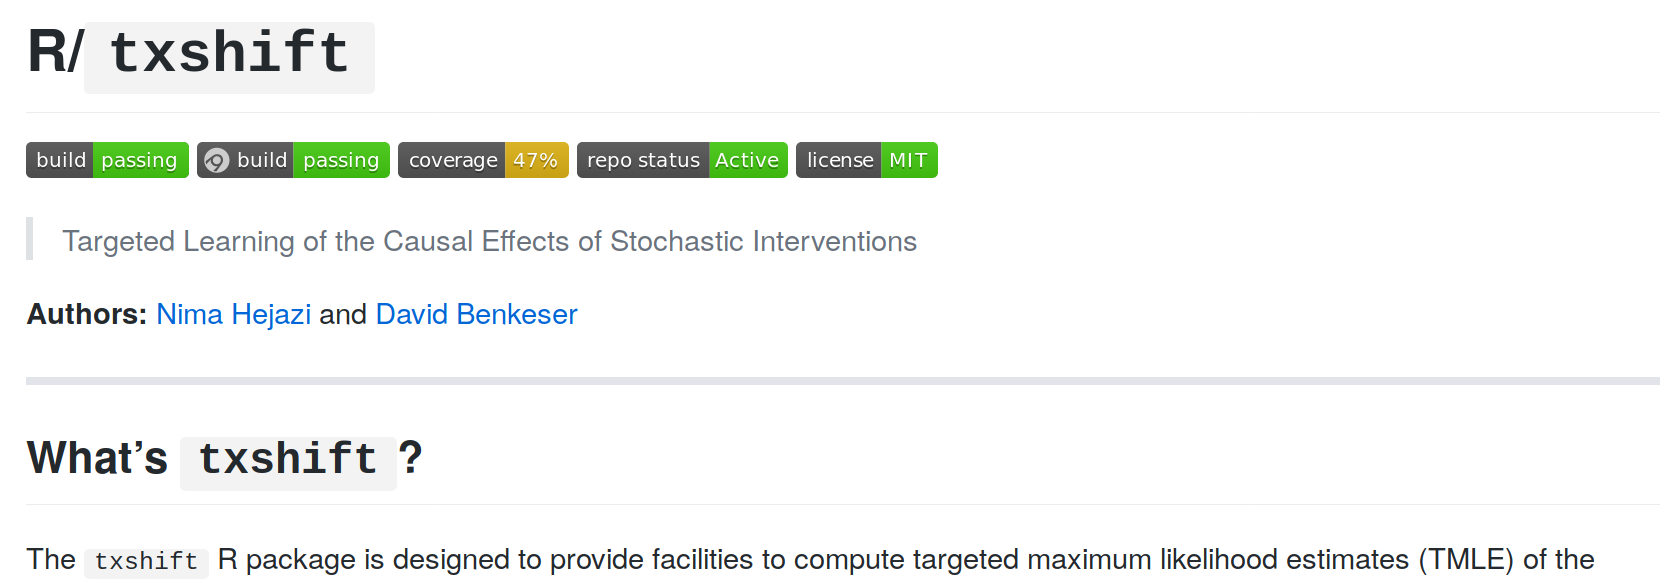
\includegraphics[width=\textwidth]{txshift}
  \caption{
    \url{https://github.com/nhejazi/txshift}
  }
\end{figure}

\vspace{-2em}

\begin{center}
\begin{itemize}
  \itemsep4pt
  \item Supports estimation of the effects of simple (additive) stochastic
    interventions.
  \item Implements both types of IPCW-TML estimator, allowing for two-phase
    sampling to be appropriately handled when $\pi_0(V)$ is known by design or
    unknown.
\end{itemize}
\end{center}

\note{
\begin{itemize}
  \itemsep10pt
  \item Contribute on GitHub: \url{https://github.com/nhejazi/txshift}.
  \item Reach out to us with questions and any feature requests.
\end{itemize}
}

\end{frame}

%%%%%%%%%%%%%%%%%%%%%%%%%%%%%%%%%%%%%%%%%%%%%%%%%%%%%%%%%%%%%%%%%%%%%%%%%%%%%%%%

\section{Extensions and Future Directions}

%%%%%%%%%%%%%%%%%%%%%%%%%%%%%%%%%%%%%%%%%%%%%%%%%%%%%%%%%%%%%%%%%%%%%%%%%%%%%%%%

\begin{frame}[c]{Ongoing Efforts}

\begin{center}
\begin{itemize}
  \itemsep10pt
  \item Extensions of stochastic interventions to causal mediation analysis ---
    new theory provides estimators of the \textit{natural direct effect} and the
    \textit{natural indirect effect}.
    \begin{itemize}
      \item Collaboration with Iv{\'a}n D{\'\i}az (Cornell) in progress.
    \end{itemize}
  \item Further refinement of the \texttt{tlverse} software ecosystem, including
    new ``connector'' \texttt{R} packages.
  \item Data analysis of the HVTN 505 HIV-1 vaccine trial, and discussion of the
    scientific findings with scientist collaborators.
\end{itemize}
\end{center}

\note{
}

\end{frame}

%%%%%%%%%%%%%%%%%%%%%%%%%%%%%%%%%%%%%%%%%%%%%%%%%%%%%%%%%%%%%%%%%%%%%%%%%%%%%%%%

\begin{frame}[c]{Future Directions}

\begin{center}
\begin{itemize}
  \itemsep10pt
  \item Exploration of different forms of stochastic interventions ---
    \cite{kennedy2018nonparametric} proposes a shift in propensity scores for
    binary (or categorical) interventions.
    \begin{itemize}
      \item Implementation in the \texttt{tlverse} ecosystem.
    \end{itemize}
  \item Refinements of statistical theory so as to better work with quantities
    common in survival analysis: hazards? survival?
  \item Assessment of newly concluded and ongoing efficacy trials through work
    with ongoing collaborators at Fred Hutch.
\end{itemize}
\end{center}

\note{
}

\end{frame}

%%%%%%%%%%%%%%%%%%%%%%%%%%%%%%%%%%%%%%%%%%%%%%%%%%%%%%%%%%%%%%%%%%%%%%%%%%%%%%%%

\begin{frame}[c]{Software and Statistics Revisited}

\begin{center}
  \begin{tabular}{ | m{5em} | m{5em}| m{2em} | m{3em} | m{2em} | }
    \hline
    \textbf{software} & \textbf{data} & \textbf{CI} & \textbf{testing} &
      \textbf{docs} \\
    \hline
    \texttt{tmle3shift} & $(W, A, Y)$ & \checkmark & \checkmark & \checkmark
      \\
    \hline
    \texttt{txshift} & $(W, A, \Delta, Y)$ & \checkmark & \checkmark &
      \checkmark \\
    \hline
    \texttt{medshift} & $(W, A, Z, Y)$ & IP & IP & IP \\
    \hline
    \texttt{tmle3} & $(W, A, Y)$ & \checkmark & \checkmark & \checkmark \\
    \hline
    \texttt{sl3} & $(X, Y)$ & \checkmark & \checkmark & \checkmark \\
    \hline
  \end{tabular}

\begin{itemize}
  \itemsep2pt
  \item Software is \textbf{not} an ancillary activity: How can a theorem or
    result impact science if no one can apply it?
  \item Writing software is important for learning statistics:
    \begin{itemize}
      \itemsep0pt
      \item How do people plan to use the software?
      \item What is the problem that the software solves?
      \item What's the ``best'' way to estimate the quantity of interest?
    \end{itemize}
  \item Writing software \textit{impacts} statistics --- minor tweaks to
    implemented estimators help us discover new ideas.
\end{itemize}
\end{center}

\note{
\begin{itemize}
  \item How I spend my time: 55\% software, 25\% writing, 10\% reading, 10\%
    simulations, 5\% data analysis.
  \item Other \texttt{R} packages: \texttt{biotmle}, \texttt{methyvim},
    \texttt{survtmle}, \texttt{survsl} (IP), \texttt{origami}, \texttt{hal9001}
\end{itemize}
}

\end{frame}

%%%%%%%%%%%%%%%%%%%%%%%%%%%%%%%%%%%%%%%%%%%%%%%%%%%%%%%%%%%%%%%%%%%%%%%%%%%%%%%%

\begin{frame}[c]{Review: Summary}

\begin{center}
\begin{itemize}
  \itemsep8pt
  \item Vaccine efficacy evaluation helps to develop enhanced vaccines better
    informed by biological properties of the target disease.
  \item HIV vaccines modulate immune responses as part of the mechanism for
    lowering HIV risk.
  \item \textit{Stochastic} interventions provide a flexible framework for
    considering \textbf{realistic} treatment policies.
  \item Large-scale vaccine trials often use two-phase sampling --- need to
    accommodate such designs.
  \item We've developed robust, open source statistical software for applying
    stochastic interventions in observational studies.
\end{itemize}
\end{center}

\note{It's always good to include a summary.}

\end{frame}

%%%%%%%%%%%%%%%%%%%%%%%%%%%%%%%%%%%%%%%%%%%%%%%%%%%%%%%%%%%%%%%%%%%%%%%%%%%%%%%%

% don't want dimming with references
\setbeamercovered{}
\beamerdefaultoverlayspecification{}

\begin{frame}[c,allowframebreaks]{}

\small
\bibliographystyle{apalike}
\nocite{*}
\bibliography{references}
%\itemize

\end{frame}

%%%%%%%%%%%%%%%%%%%%%%%%%%%%%%%%%%%%%%%%%%%%%%%%%%%%%%%%%%%%%%%%%%%%%%%%%%%%%%%%

\begin{frame}{Acknowledgments}

\vspace{20pt}

\underline{Close Collaborators and Advisors:}\\
\hspace{0.15cm}
\begin{tabular}{@{}l@{\hspace{0.75cm}}l@{\vspace{0.5em}}}
  Mark J.~van der Laan & University of California,
    Berkeley \\
  Alan E.~Hubbard & University of California,
    Berkeley \\
  David C.~Benkeser & Emory University \\
  Jeremy R.~Coyle & University of California,
    Berkeley \\
  Peter B.~Gilbert & Fred Hutchinson Cancer Research
    Center \\
  Holly E.~Janes & Fred Hutchinson Cancer Research Center
\end{tabular}

\end{frame}

%%%%%%%%%%%%%%%%%%%%%%%%%%%%%%%%%%%%%%%%%%%%%%%%%%%%%%%%%%%%%%%%%%%%%%%%%%%%%%%%

\begin{frame}[c]{Thank you.}

\vspace{2mm}

\includegraphics[scale=0.14]{homepage.png} \url{https://nimahejazi.org}

\vspace{2mm}

\includegraphics[scale=0.11]{github-icon.png}
  \url{https://github.com/nhejazi}

\vspace{2mm}

\includegraphics[scale=0.14]{twitter-icon.png}
  \url{https://twitter.com/nshejazi}

\end{frame}

%%%%%%%%%%%%%%%%%%%%%%%%%%%%%%%%%%%%%%%%%%%%%%%%%%%%%%%%%%%%%%%%%%%%%%%%%%%%%%%%

\appendix
\begin{frame}[standout]
  Appendix
\end{frame}

%%%%%%%%%%%%%%%%%%%%%%%%%%%%%%%%%%%%%%%%%%%%%%%%%%%%%%%%%%%%%%%%%%%%%%%%%%%%%%%%

\begin{frame}[c]{Literature: \cite{diaz2012population}}

\begin{center}
\begin{itemize}
  \itemsep10pt
  \item \textit{Proposal:} Evaluate outcome under an altered
    \textit{intervention distribution} --- e.g.,
    $P_{\delta}(g_0)(A = a \mid W) = g_0(a - \delta(W) \mid W)$.
  \item Identification conditions for a statistical parameter of the
    counterfactual outcome $\psi_{0,d}$ under such an intervention.
  \item Show that the causal quantity of interest $\E_0 \{Y_{d(A, W)}\}$ is
    identified by a functional of the distribution of $X$:
    \begin{align*}\label{eqn:identification2012}
      \psi_{0,d} = \int_{\mathcal{W}} \int_{\mathcal{A}} &\E_{P_0^X} \{Y \mid
        A = d(a, w), W = w\} \cdot \\ &q_{0, A}^X(a \mid W = w) \cdot
        q_{0, W}^X(w) d\mu(a)d\nu(w)
    \end{align*}
  \item Provides a derivation based on the efficient influence function (EIF)
    with respect to the nonparametric model $\mathcal{M}$.
\end{itemize}
\end{center}

\note{
  \begin{itemize}
    \item The identification result allows us to write down the causal quantity
      of interest in terms of a functional of the observed data.
    \item Key innovation: loosening standard assumptions through a change in
      the observed intervention mechanism.
    \item Problem: globally altering an intervention mechanism does not
      necessarily respect individual characteristics.
    \item The authors build IPW, A-IPW, and TML estimators, comparing the three
      different approaches.
    \item IMPORTANT: gives the g-computation formula for identification of this
      estimator from the observed data structure.
  \end{itemize}
}

\end{frame}

%%%%%%%%%%%%%%%%%%%%%%%%%%%%%%%%%%%%%%%%%%%%%%%%%%%%%%%%%%%%%%%%%%%%%%%%%%%%%%%%

\begin{frame}[c]{Literature: \cite{haneuse2013estimation}}

\begin{center}
\begin{itemize}
  \itemsep10pt
  \item \textit{Proposal:} Characterization of stochastic interventions as
    \textit{modified treatment policies} (MTPs).
  \item Assumption of \textit{piecewise smooth invertibility} allows for the
    intervention distribution of any MTP to be recovered:
    \begin{equation*}
      g_{0, \delta}(a \mid w) = \sum_{j = 1}^{J(w)} I_{\delta, j} \{h_j(a, w),
      w\} g_0\{h_j(a, w) \mid w\} h^{'}_j(a,w)
    \end{equation*}
  \item Such intervention policies account for the natural value of the
    intervention $A$ directly yet are interpretable as the imposition of an
    altered intervention mechanism.
  \item Identification conditions for assessing the parameter of interest under
    such interventions appear technically complex (at first).
\end{itemize}
\end{center}

\note{
  \begin{itemize}
    \item Shifts of the form $d(A,W)$ are considerably more interesting since
      these are realistic intervention policies.
    \item Example: consider an individual with an extremely high immune response
      but whose baseline covariates $W$ suggest we shift the response still
      higher. Such a shift may not be biologically plausible (impossible, even)
      but we cannot account for this if the shift is only a function of $W$.
    \item The authors build IPW, outcome regression, and non-iterative doubly
      robust estimators, as well as an approach based on MSMs.
    \item Piecewise smooth invertibility: This assumption ensures that we can
      use the change of variable formula when computing integrals over $A$ and
      it is useful to study the estimators that we propose in this paper.
  \end{itemize}
}

\end{frame}

%%%%%%%%%%%%%%%%%%%%%%%%%%%%%%%%%%%%%%%%%%%%%%%%%%%%%%%%%%%%%%%%%%%%%%%%%%%%%%%%

\begin{frame}[c]{Literature: \cite{young2014identification}}

\begin{center}
\begin{itemize}
  \itemsep10pt
  \item Establishes equivalence between g-formula when proposed intervention
    depends on natural value and when it does not.
  \item This equivalence leads to a sufficient positivity condition for
    estimating the counterfactual mean under MTPs via the same statistical
    functional studied in \cite{diaz2012population}.
  \item Extends earlier identification results, providing a way to use the same
    statistical functional to assess $\E Y_{d(A,W)}$ or $\E Y_{d(W)}$.
  \item The authors also consider limits on implementing shifts $d(A,W)$, and
    address working in a longitudinal setting.
\end{itemize}
\end{center}

\note{
}

\end{frame}

%%%%%%%%%%%%%%%%%%%%%%%%%%%%%%%%%%%%%%%%%%%%%%%%%%%%%%%%%%%%%%%%%%%%%%%%%%%%%%%%

\begin{frame}[c]{Literature: \cite{diaz2018stochastic}}

\begin{center}
\begin{itemize}
  \itemsep10pt
  \item Builds on the original proposal, accomodating MTP-type shifts $d(A,W)$
    proposed after their earlier work.
  \item To protect against positivity violations, considers a specific shifting
    mechanism:
     \begin{equation*}\label{shift_intervention}
       d(a, w) =
         \begin{cases}
           a + \delta, & a + \delta < u(w) \\
           a, & \text{otherwise}
         \end{cases}
     \end{equation*}
  \item Proposes an improved ``1-TMLE'' algorithm, with a single auxiliary
    covariate for constructing the TML estimator.
  \item Our (first) contribution: implementation of this algorithm.
\end{itemize}
\end{center}

\note{
}

\end{frame}

%%%%%%%%%%%%%%%%%%%%%%%%%%%%%%%%%%%%%%%%%%%%%%%%%%%%%%%%%%%%%%%%%%%%%%%%%%%%%%%%

\begin{frame}[c]{Nonparametric Conditional Density Estimation}

\begin{center}
\begin{itemize}
  \itemsep8pt
  \item To compute the auxiliary covariate $H(a,w)$, we need to estimate
    conditional densities $g(A \mid W)$ and $g(A - \delta \mid W)$.
  \item There is a rich literature on density estimation, we follow the approach
    proposed in \cite{diaz2011super}.
  \item To build a conditional density estimator, consider
    \begin{equation*}
      g_{n, \alpha}(a \mid W) = \frac{\pr (A \in [\alpha_{t-1}, \alpha_t)
        \mid W)}{\alpha_t - \alpha_{t-1}},
    \end{equation*}
    for $\alpha_{t-1} \leq a < \alpha_t$.
    \vspace{0.5em}
    \begin{itemize}
      \itemsep4pt
      \item This is a classification problem, where we estimate the probability
        that a value of $A$ falls in a bin $[\alpha_{t-1}, \alpha_t)$.
      \item The choice of the tuning parameter $t$ corresponds roughly to the
        choice of bandwidth in classical kernel density estimation.
    \end{itemize}
\end{itemize}
\end{center}

\note{
}

\end{frame}

%%%%%%%%%%%%%%%%%%%%%%%%%%%%%%%%%%%%%%%%%%%%%%%%%%%%%%%%%%%%%%%%%%%%%%%%%%%%%%%%

\begin{frame}[c]{Nonparametric Conditional Density Estimation}

\begin{center}
\begin{itemize}
  \itemsep8pt
  \item \cite{diaz2011super} propose a re-formulation of this classification
    approach as a set of hazard regressions.
  \item To effectively employ this proposed re-formulation, consider
    \begin{align*}
      \pr (A \in [\alpha_{t-1}, \alpha_t) \mid W) =& \pr (A \in [\alpha_{t-1},
      \alpha_t) \mid A \geq \alpha_{t-1}, W) \times  \\ & \Pi_{j = 1}^{t -1}
      \{1 - \pr (A \in [\alpha_{j-1}, \alpha_j) \mid A \geq \alpha_{j-1}, W) \}
    \end{align*}
    \vspace{0.25em}
    \begin{itemize}
      \itemsep4pt
      \item The likelihood of this model may be expressed to correspond to the
        likelihood of a binary variable in a data set expressed via a long-form
        repeated measures structure.
      \item Specifically, the observation of $X_i$ is repeated as many times as
        intervals $[\alpha_{t-1}, \alpha_t)$ are before the interval to which
        $A_i$ belongs, and the binary variables indicating $A_i \in
        [\alpha_{t-1}, \alpha_t)$ are recorded.
    \end{itemize}
\end{itemize}
\end{center}

\note{
}

\end{frame}

%%%%%%%%%%%%%%%%%%%%%%%%%%%%%%%%%%%%%%%%%%%%%%%%%%%%%%%%%%%%%%%%%%%%%%%%%%%%%%%%

\begin{frame}[c]{Density Estimation with the Super Learner Algorithm}

\begin{center}
\begin{itemize}
  \itemsep10pt
  \item To estimate $g(A \mid W$) and $g(A - \delta \mid W)$, use a pooled
    hazard regression, spanning the support of $A$.
  \item We rely on the Super Learner algorithm of \cite{vdl2007super} to build
    an ensemble learner that optimally weights each of the proposed regressions,
    using cross-validation (CV).
  \item The Super Learner algorithm uses $V$-fold CV to train each proposed
    regression model, weighting each by the inverse of its average risk across
    all $V$ holdout sets.
  \item By using a library of regression estimators, we invoke the result of
    \cite{vdl2004asymptotic}, who prove this likelihood-based cross-validated
    estimator to be asymptotically optimal.
\end{itemize}
\end{center}

\note{
\begin{itemize}
  \item The auxiliary covariate simplifies when the treatment is in the limits
    (conditional on $W$) --- i.e., for $A_i \in (u(w) - \delta, u(w))$, then we
    have $H(a,w) = \frac{g_0(a - \delta \mid w)}{g_0(a \mid w)} + 1$.
  \item Asymptotically optimal in the sense that it performs as well as the
    oracle selector as the sample size increases.
\end{itemize}
}

\end{frame}

%%%%%%%%%%%%%%%%%%%%%%%%%%%%%%%%%%%%%%%%%%%%%%%%%%%%%%%%%%%%%%%%%%%%%%%%%%%%%%%%

\begin{frame}[c]{Algorithm for IPCW-TML Estimation}

\begin{center}
\begin{enumerate}\label{ipcwtmle_algo}
  \itemsep8pt
  \item Using all observed units ($X$), estimate sampling mechanism
    $\pi(Y, W)$, perhaps using data-adaptive regression methods.
  \item Using only observed units in the second-stage sample $\Delta = 1$,
    construct initial estimators $g_n(A, W)$ and $\overline{Q}_n(A, W)$,
    weighting by the sampling mechanism estimate $\pi_n(Y, W)$.
  \item With the approach described for the full data case, compute
    $H_n(a_i,w_i)$, and fluctuate submodel via logistic regression.
  \item Compute IPCW-TML estimator $\Psi_n$ of the target parameter, by solving
    the IPCW-augmented EIF estimating equation.
  \item Iteratively update estimated sampling weights $\pi_n(Y,W)$ and
    IPCW-augmented EIF, updating TML estimate in each iteration, until
    $\frac{1}{n}\sum_{i = 1}^n \text{EIF}_i < \frac{1}{n}$.
\end{enumerate}
\end{center}

\note{
  \begin{itemize}
    \item We recommend using nonparametric methods for the initial estimators,
      as consistent estimation is necessary for efficiency of the estimator
      $\Psi_n$.
    \item Intuition for the submodel fluctuation?
    \item This process includes the use of HAL to fit the regression of the EIF
      contributions on the sampling node $\{Y, W\}$.
  \end{itemize}
}

\end{frame}

%%%%%%%%%%%%%%%%%%%%%%%%%%%%%%%%%%%%%%%%%%%%%%%%%%%%%%%%%%%%%%%%%%%%%%%%%%%%%%%%

\begin{frame}[c]{A Realistic Shift Intervention}

\begin{center}

Consider a more sophisticated shift function:

\begin{equation*}
  \delta(a, w) =
    \begin{cases}
      \delta, & \delta_{\text{min}}(a,w) \leq \delta \leq
        \delta_{\text{max}}(a,w) \\
      \delta_{\text{max}}(a,w), & \delta \geq \delta_{\text{max}}(a,w) \\
      \delta_{\text{min}}(a,w), & \delta \leq \delta_{\text{min}}(a,w) \\
    \end{cases},
\end{equation*}
where we define maximal and minimal possible shifts:
$$\delta_{\text{max}}(a, w) = \text{argmax}_{\left\{\delta \geq 0,
\frac{g(a - \delta \mid w)}{g(a \mid w)} \leq M \right\}} \frac{g(a - \delta
\mid w)}{g(a \mid w)}$$ and
$$\delta_{\text{min}}(a, w) = \text{argmin}_{\left\{\delta \leq 0,
\frac{g(a - \delta \mid w)}{g(a \mid w)} \leq M \right\}} \frac{g(a - \delta
\mid w)}{g(a \mid w)}.$$
\end{center}

\note{
}

\end{frame}

%%%%%%%%%%%%%%%%%%%%%%%%%%%%%%%%%%%%%%%%%%%%%%%%%%%%%%%%%%%%%%%%%%%%%%%%%%%%%%%%

\begin{frame}[c]{Variable Importance Analysis with MSMs}

\begin{center}
\begin{itemize}
  \itemsep10pt
  \item Consider now a grid of $j$ possible shift values $\delta$, where we seek
    to estimate the counterfactual mean under each value of $\delta$.
  \item With this approach, we construct $j$ estimates $\psi_{n,j}$ of the
    counterfactual mean, each under a different proposed value of the shift
    $\delta_j$.
  \item We may summarize $\psi_{n,j}$ through a working marginal structural
    model (MSM), constructing inference through a hypothesis test of the a
    parameter of the MSM.
  \item Formally, let $\vec{\psi}_{\delta} = (\psi_{\delta}: \delta)$ with
    corresponding estimators $\vec{\psi}_{n, \delta} = (\psi_{n, \delta}:
    \delta)$. Further, let $\beta(\vec{\psi}_{\delta}) = \phi((\psi_{\delta}:
    \delta))$
\end{itemize}
\end{center}

\note{
}

\end{frame}

%%%%%%%%%%%%%%%%%%%%%%%%%%%%%%%%%%%%%%%%%%%%%%%%%%%%%%%%%%%%%%%%%%%%%%%%%%%%%%%%

\begin{frame}[c]{Variable Importance Analysis with MSMs}

\begin{center}
\begin{itemize}
  \itemsep10pt
  \item For a given MSM $m_{\beta}(\delta)$, we have that
    $$\beta_0 = \text{argmin}_{\beta} \sum_{\delta}(\psi_{\delta}(P_0) -
    m_{\beta}(\delta))^2 h(\delta),$$
  \item This then leads to the following expansion
    $$\beta(\vec{\psi}_n) - \beta(\vec{\psi}_0) \approx -\frac{d}{d\beta}
    u(\beta_0, \vec{\psi}_0)^{-1} \frac{d}{d\psi} u(\beta_0,
    \psi_0)(\vec{\psi}_n - \vec{\psi}_0),$$
  \item In terms of the efficient influence function (EIF) of $\psi$ by using
    the first order approximation $(\psi_n - \psi_0)(\delta) =
    \frac{1}{n}\sum_{i = 1}^n \text{EIF}_{\psi_{\delta}}(O_i)$, where
    $\text{EIF}_{\psi_{\delta}}$ is the efficient influence function (EIF) of
    $\vec{\psi}$
\end{itemize}
\end{center}

\note{
}

\end{frame}

%%%%%%%%%%%%%%%%%%%%%%%%%%%%%%%%%%%%%%%%%%%%%%%%%%%%%%%%%%%%%%%%%%%%%%%%%%%%%%%%

\begin{frame}[c]{Variable Importance Analysis with MSMs}

\begin{center}
\begin{itemize}
  \itemsep10pt
  \item Now, say, $\vec{\psi} = (\psi(\delta): \delta)$ is d-dimensional, then
    we may write the efficient influence function of the MSM parameter $\beta$
    (assuming a linear MSM) as follows
    \begin{align*}
      \text{EIF}_{\beta}(O) =& \left(\sum_{\delta} h(\delta) \frac{d}{d\beta}
      m_{\beta}(\delta) \frac{d}{d\beta} m_{\beta}(\delta)^t \right)^{-1}
      \cdot \\ &\sum_{\delta} h(\delta) \frac{d}{d\beta} m_{\beta}(\delta)
      \text{EIF}_{\psi_{\delta}}(O),
    \end{align*}
    where the first term is of dimension $d \times d$ and the second term is of
    dimension $d \times 1$.
\end{itemize}
\end{center}

\note{
}

\end{frame}

%%%%%%%%%%%%%%%%%%%%%%%%%%%%%%%%%%%%%%%%%%%%%%%%%%%%%%%%%%%%%%%%%%%%%%%%%%%%%%%%

\end{document}

